\begin{defn}[Statements]
    A \emph{statement}\index{statement} (or \emph{proposition}\index{proposition}) is a sentence which is true or false but not both.
\end{defn}
\begin{defn}[New Statements From Old]
    Given statements \(P\) and \(Q\):
    \begin{itemize}
        \item The \emph{negation}\index{negation} of a statement, \(\sim P\) or \(not\ P\), always has the opposite truth value.
        \item The \emph{conjunction}\index{conjunction} of two statements, \(P\wedge Q\) or \(P\ and\ Q\), is true when both statements are true.
        \item The \emph{disjunction}\index{disjunction} of two statements, \(P\vee Q\) or \(P\ or\ Q\), is true when either statement is true.
        % \item A \emph{conditional statement} with two statements, \(P\rightarrow Q\) or \(if\ P\ then \ Q\), is false when \(P\) is true and \(Q\) is false, it is otherwise true.
    \end{itemize}
\end{defn}


\begin{practiceprob}[Statements and Their Negations]\label{rainstatements}
    Fill in the negation for the statements: \(R\equiv\) ``It is raining.''; \(G\equiv\) ``The grass is wet.''; and \(U\equiv\) ``I have an umbrella.''
        \begin{itemize}
            \item \(\sim R\equiv\) \vspace{\baselineskip}
            \item \(\sim G\equiv\) \vspace{\baselineskip}
            \item \(\sim U\equiv\) \vspace{\baselineskip}
        \end{itemize}
\end{practiceprob}

\clearpage

\newcounter{n}
\setcounter{n}{1}
\begin{practiceprob}[Visualizing Truth Values]\label{mainimages}
    For each picture indicate all the statements from practice problem \ref{rainstatements} that apply to it by writing the appropriate letter or its negation.
    \begin{center}
        % \inputtikz{grass_zombies}
        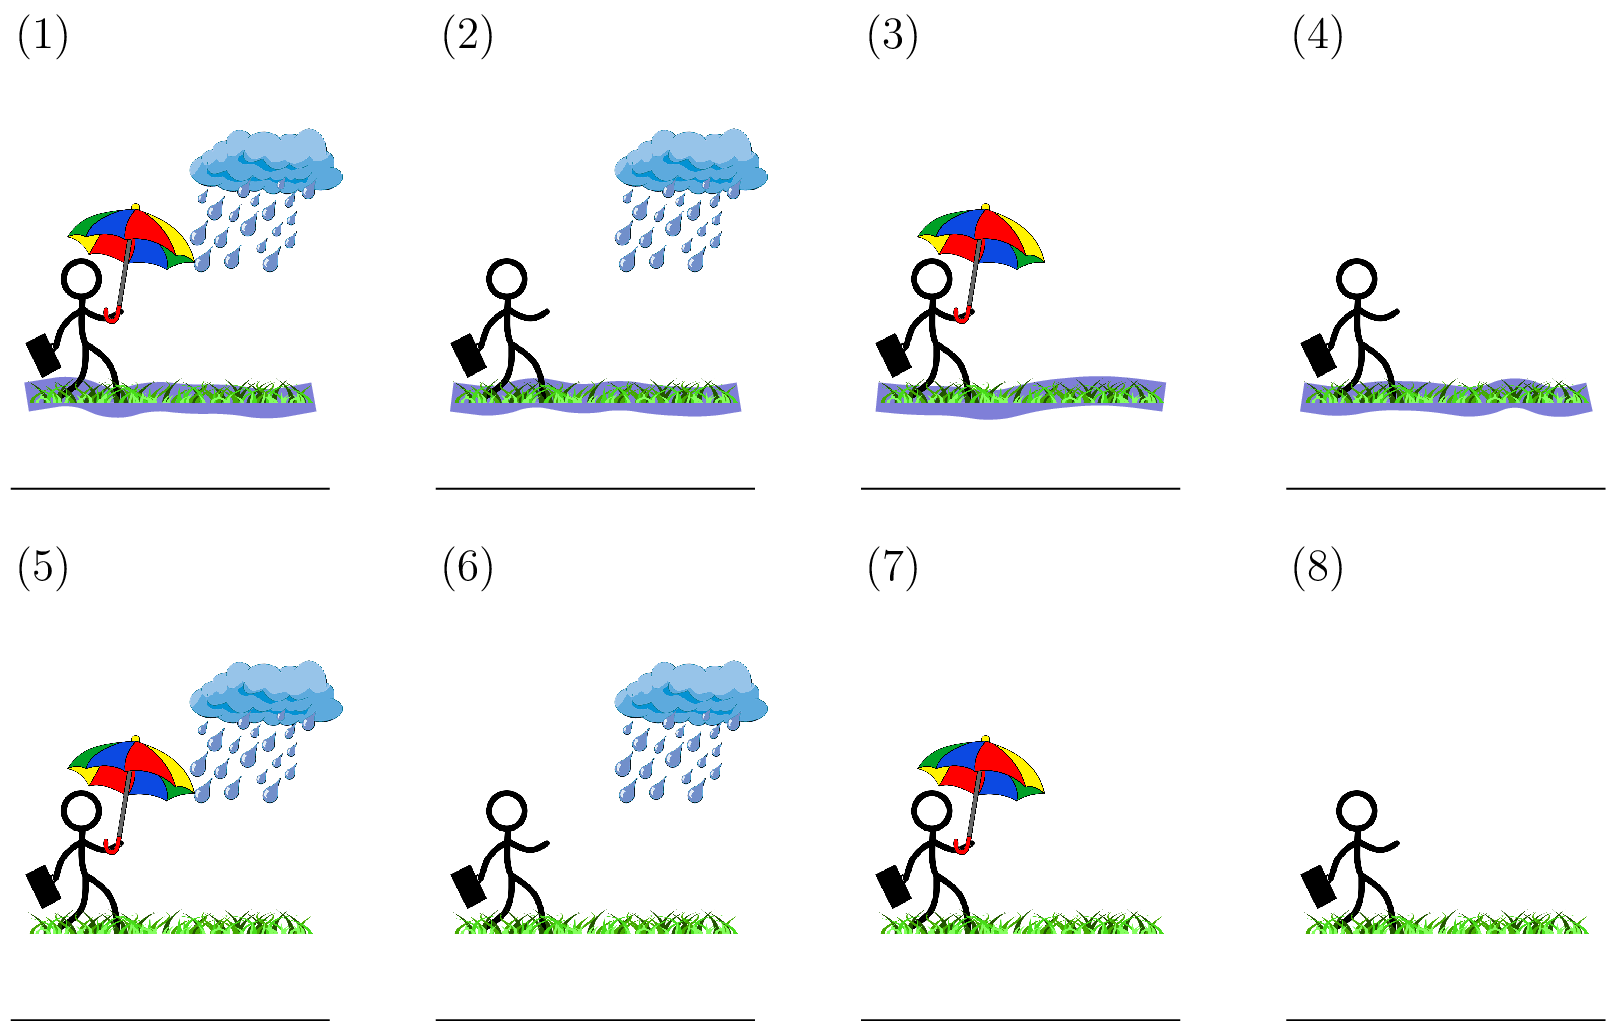
\includegraphics[scale=0.24,alt={Eight images with different configurations of a stick figure with out without rain or an umbrella or wet grass.},width=0.85\linewidth]{images/created/grass_zombies.png}
    \end{center}
\end{practiceprob}



\begin{practiceprob}[Relating Statements to Sets]
    For each region of the Venn Diagram, write down which picture from practice problem \ref{mainimages} belongs in that region.
    \begin{center}
        % \inputtikz{venn_zombies}
        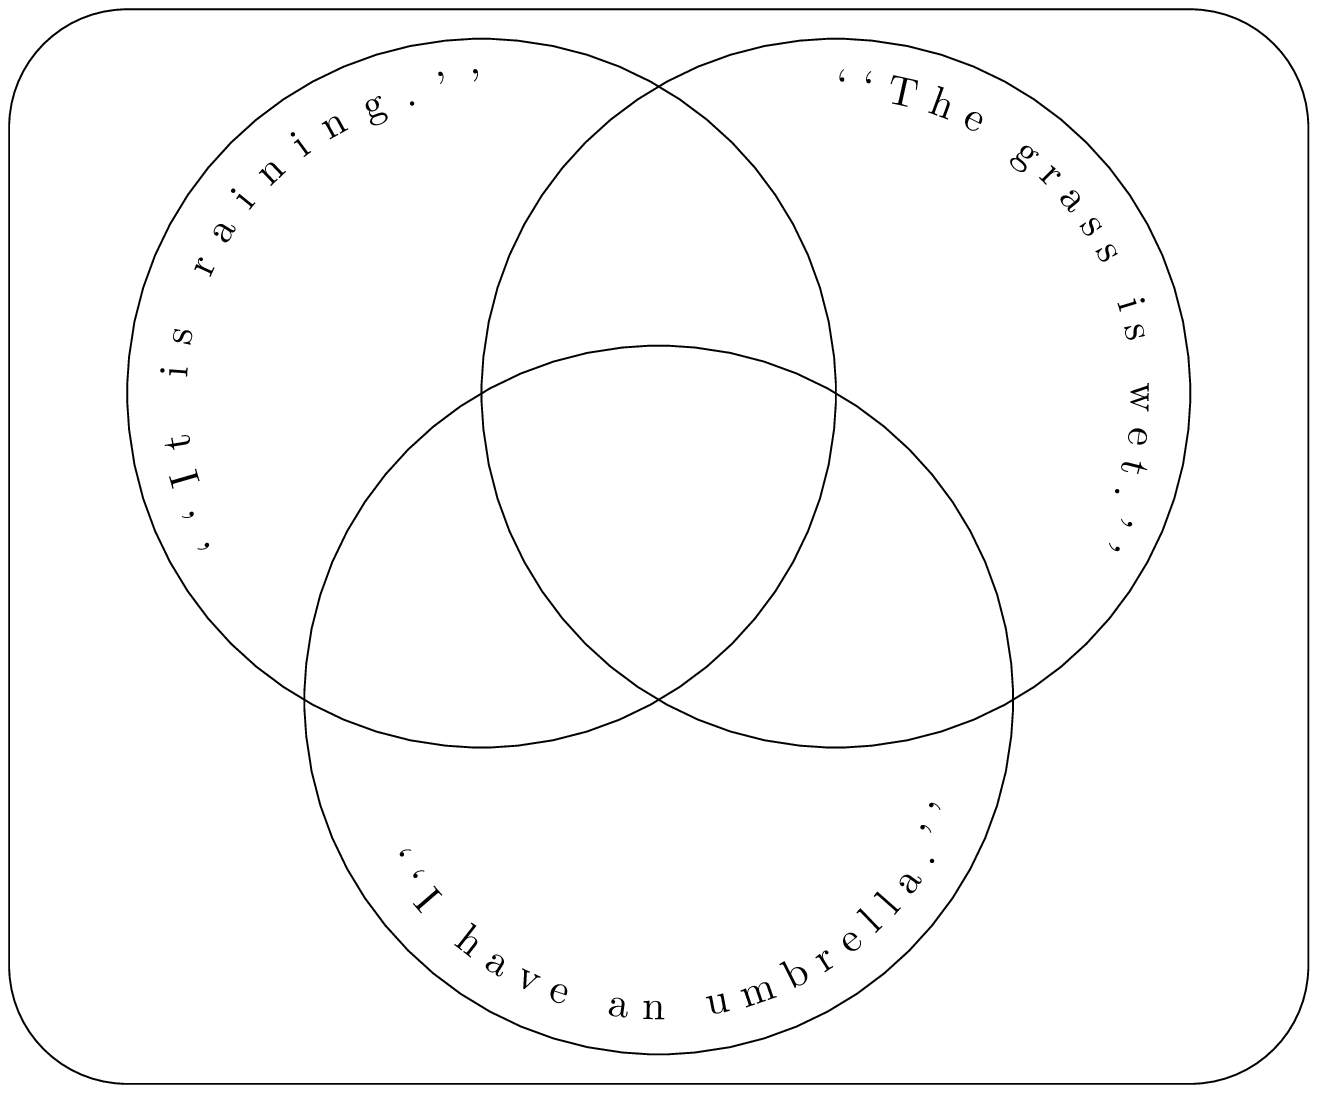
\includegraphics[scale=0.24,alt={Blank Venn diagram for organizing the previous images into three overlapping sets.},width=0.65\linewidth]{images/created/venn_zombies.png}        
    \end{center}    
\end{practiceprob}

\clearpage

\begin{practiceprob}[Combinations and Modifications of Statements]
    For each combination of statements, indicate which set of pictures from practice problem \ref{mainimages} make the statement true.
    \begin{multicols}{2}
    \begin{enumerate}
    \setlength{\itemsep}{10pt}
        \item \(U\wedge G\): 
        \item \(\sim(U\wedge G)\): 
        \item \(\sim U\wedge \sim G\): 
        \item \(U\vee G\): 
        \item \(\sim(U\vee G)\): 
        \item \(\sim U \vee \sim G\): 
    \end{enumerate}   
    \end{multicols}
\end{practiceprob}

\begin{practiceprob}[Negating Compound Statements]
    \setlength{\extrarowheight}{10pt}
    Using \(U\equiv\) ``I have an umbrella.'' and \(G\equiv\) ``The grass is wet.'' fill in the \emph{truth table} below.  You can refer to the previous practice problems and the images above to help you.
    \begin{center}
    \begin{tabular}{*{4}{c}*{5}{>{\centering}m{0.125\textwidth}}}
        \(U\) & \(G\) & \(\sim U\) & \(\sim G\) & \(U\wedge G\) & \(U\vee G\) & \(\sim (U\wedge G)\) & \(\sim (U\vee G)\) & \(U \wedge \sim G\) \tabularnewline\hline
        \(T\)&\(T\)&&&&&&&\tabularnewline\hline
        \(T\)&\(F\)&&&&&&&\tabularnewline\hline
        \(F\)&\(T\)&&&&&&&\tabularnewline\hline
        \(F\)&\(F\)&&&&&&&\tabularnewline\hline        
    \end{tabular}
    \end{center}
\end{practiceprob}



\begin{defn}[Tautology and Contradiction]
    A \emph{tautology}\index{tautology} is a statement that is always true and a \emph{contradiction}\index{contradiction} is a statement that is always false.  For example, in the figures in practice problem \ref{mainimages}, ``the grass is green'' is a tautology since it is always true, ``there is a zombie'' is a contradiction since it is always false.
\end{defn}

\begin{practiceprob}[True or False]
    For which pictures in practice problem \ref{mainimages} are the following sentences true?
    \begin{enumerate}
    \setlength{\itemsep}{10pt}
        \item ``The grass is green.'' 
        \item ``There is a zombie.'' 
        \item ``The grass is green'' \(\vee\) ``I have an umbrella.'' 
        % \item ``The grass is green'' \(\wedge\) ``I have an umbrella.'' 
        % \item ``There is a zombie'' \(\vee\) ``I have an umbrella.'' 
        \item ``There is a zombie'' \(\wedge\) ``I have an umbrella.'' 
        \item ``There is a zombie'' \(\vee\) ``the grass is green.'' 
        \item ``There is a zombie'' \(\wedge\) ``the grass is green.'' 
    \end{enumerate}    
\end{practiceprob}

\begin{exposition}{Some ``Basic'' Logical Rules}
So far we have identified the following ways to put together statements using \(\wedge\), \(\vee\), and \(\sim\):
\begin{itemize}
    \setlength{\itemsep}{25pt}
    \begin{multicols}{2}
        \item \emph{Negation (not)}\index{negation}: \(\sim P\)
        \item \emph{Conjunction (and)}\index{conjunction}: \(P\wedge Q\)
        \item \emph{Disjunction (or)}\index{disjunction}: \(P \vee Q\)
        \item \emph{Exclusive Or (xor)}\index{exclusive or}\index{exclusive or!xor}:\newline \(P \oplus Q \equiv (P\vee Q) \wedge \sim(P\wedge Q)\)
        \item \emph{Double Negation}\index{double negation}: \(\sim(\sim P)\equiv P\)
        \item \emph{DeMorgan's Laws}\index{Demorgan's Laws}: 
        \begin{itemize}
            \item \(\sim(P\wedge Q)\equiv \sim P \vee \sim Q\)
            \item \(\sim(P\vee Q)\equiv \sim P \wedge \sim Q\)
        \end{itemize}
        \item \emph{Commutative Law}\index{commutative law}: 
        \begin{itemize}
            \item \(P\vee Q\equiv Q \vee P\)
            \item \(P\wedge Q\equiv Q \wedge P\)
        \end{itemize}
\columnbreak
        \item \emph{Distributive Law}\index{distributive law}: 
        \begin{itemize}
            \item \(P\wedge (Q\vee R)\equiv P\wedge Q \vee P\wedge R\)
            \item \(P\vee (Q\wedge R)\equiv P\vee Q \wedge P\vee R\)
        \end{itemize}
        \item \emph{Associative Law}\index{associative law}: 
        \begin{itemize}
            \item \(P\wedge (Q\wedge R)\equiv (P\wedge Q) \wedge R\)
            \item \(P\vee (Q\vee R)\equiv (P\vee Q) \vee R\)
        \end{itemize}
        \item \emph{Identity Laws}\index{identity laws}:
        \begin{itemize}
            \item \(t \wedge P \equiv P\)
            \item \(c \vee P \equiv P\)
        \end{itemize}
        \item \emph{Inverse Laws}\index{inverse laws}:
        \begin{itemize}
            \item \(P \vee \sim P \equiv t\)
            \item \(P \wedge \sim P \equiv c\)
        \end{itemize}
        \item \emph{Domination Laws}\index{domination laws}:
        \begin{itemize}
            \item \(t \vee P \equiv t\)
            \item \(c \wedge P \equiv c\)
        \end{itemize}
    \end{multicols}
\end{itemize}
\index{laws!double negation}
\index{laws!DeMorgan's}
\index{laws!commutative}
\index{laws!distributive}
\index{laws!associative}
\index{laws!identity}
\index{laws!inverse}
\index{laws!domination}
\end{exposition}